\section{MHS}

\begin{frame}{Oscilações -- Lei de Hooke}
    \begin{center}
        \begin{tikzpicture}[
            ground/.style={fill,pattern=north east lines,draw=none,minimum width=0.3,minimum height=0.6},
            spring/.style={line width=0.8,blue!7!black!80,decorate, decoration={coil,amplitude=5,segment length=5},line cap=round},
            mass/.style={line width=0.6,red!30!black,fill=red!40!black!10,rounded corners=1,
            top color=red!40!black!20,bottom color=red!40!black!10,shading angle=20}
            ]
            \def\H{1}    % wall height
            \def\T{0.3}  % wall thickness
            \def\W{5.0}  % ground length
            \def\D{0.25} % ground depth
            \def\h{0.6}  % mass height
            \def\w{0.7}  % mass width
            \def\x{1.6}  % mass x position

            \foreach \y/\x in {0/2.0,1.5/1.0,3/3.0} {
                \begin{scope}[shift={(0,-\y)}]
                    \draw[spring] (0,\h/2) --++ (\x,0);
                    \draw[ground] (0,0) |-++ (-\T,\H) |-++ (\T+\W,-\H-\D) -- (\W,0) -- cycle;
                    \draw (0,\H) -- (0,0) -- (\W,0);
                    \draw[mass] (\x,0) rectangle++ (\w,\h) node[midway] {$m$};
                \end{scope}
            }
            \node [red] at (\W,\h/2) {$\phantom{\rightarrow~}F=0$};
            \node [red] at (\W,\h/2-1.5) {$\rightarrow~F>0$};
            \node [red] at (\W,\h/2-3) {$\leftarrow~F<0$};
        \end{tikzpicture}
    \end{center}

    \[
        F = -kx \rightarrow
        \begin{cases}
            F = 0, \text{ se } x =0\\
            F > 0, \text{ se } x<0\\
            F < 0, \text{ se } x>0
        \end{cases}
        \rightarrow
        \text{Força restauradora}
    \]
\end{frame}

\begin{frame}{Equação diferencial}
    \[
        F=-kx \implies ma=-kx \implies m\frac{d^2 x}{dt^2}=-kx \implies \frac{d^2 x}{dt^2}=-\frac{k}{m} x
    \]
    \begin{gather*}
    \Downarrow \\
    \boxed{\color{blue} \frac{d^2 u}{dt^2}= -\omega^2 u \implies \text{Movimento Harmônico Simples}}
    \end{gather*}
    Solução geral:
    \[
        u=C_1 \sen{\omega t} + C_2 \cos{\omega t} \implies
        \begin{cases}
            A \sin{(\omega t + \delta)} \\
            A \cos{(\omega t + \delta)}
        \end{cases}
        \implies A \cos{(\omega t + \delta)}
    \]
\end{frame}

\begin{frame}{Gráfico de \(u=A \cos{(\omega t+\delta)}\)}
    \begin{columns}[c]
        \begin{column}{0.6\textwidth}
            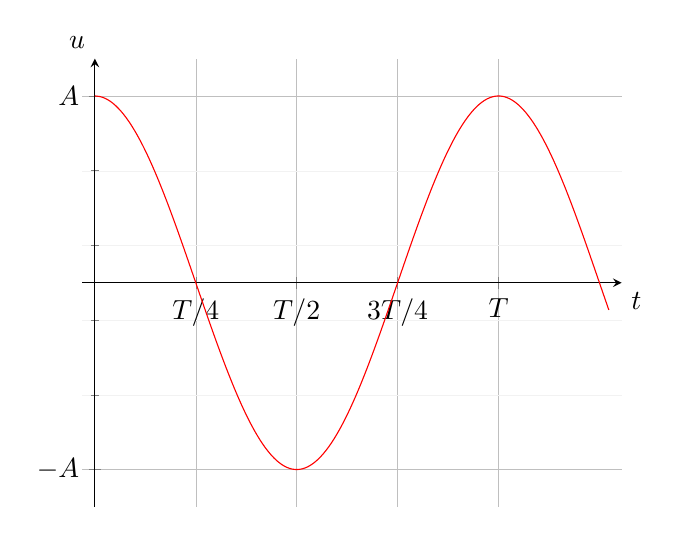
\begin{tikzpicture}
                \begin{axis}%
                    [grid=both,
                    minor tick num=4,
                    grid style={line width=.1pt, draw=gray!10},
                    major grid style={line width=.2pt,draw=gray!50},
                    axis lines=middle,
                    enlargelimits={abs=0.2},
                    xlabel={$t$},
                    ylabel={$u$},
                    xlabel style={below right},
                    ylabel style={above left},
                    xtick={pi/2,pi,3*pi/2, 2*pi},
                    xticklabels={$T/4$,$T/2$,$3T/4$,$T$},
                    ytick={-1,1},
                    yticklabels={$-A$,$A$}
                    ]
                    \addplot[domain=0:8,samples=100,smooth,red] {cos(deg(x))};
                \end{axis}
            \end{tikzpicture}
        \end{column}

        \begin{column}{0.4\textwidth}
            \begin{itemize}
                \item \(A\) é a amplitude
                \item \(T\) é o período e \(T=2\pi/\omega\)
                \item \(\omega t + \delta\) é a fase
                \item \(\delta\) é a constante de fase
                \item \(\omega\) é a frequência angular
                \item \(f\) é a frequência e \(\omega = 2\pi f\)
                    \[
                        \color{blue}
                        T=\frac{1}{f}
                    \]
            \end{itemize}
            \begin{tcolorbox}[colback=blue!10]
                No SI, T é em \si{s}, \(\omega\) é em \si{rad/s} e f é em \si{Hz} (ciclo/s)
            \end{tcolorbox}
        \end{column}
    \end{columns}
\end{frame}

\begin{frame}{A constante de fase}
    \centering
    \begin{columns}[c]
        \begin{column}{0.45\textwidth}
            \[\delta = 0\]
            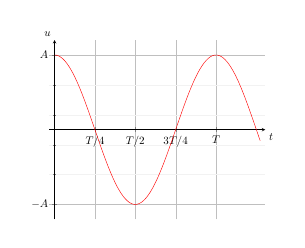
\begin{tikzpicture}[scale=0.4]
                \begin{axis}%
                    [grid=both,
                    minor tick num=4,
                    grid style={line width=.1pt, draw=gray!10},
                    major grid style={line width=.2pt,draw=gray!50},
                    axis lines=middle,
                    enlargelimits={abs=0.2},
                    xlabel={$t$},
                    ylabel={$u$},
                    xlabel style={below right},
                    ylabel style={above left},
                    xtick={pi/2,pi,3*pi/2, 2*pi},
                    xticklabels={$T/4$,$T/2$,$3T/4$,$T$},
                    ytick={-1,1},
                    yticklabels={$-A$,$A$}
                    ]
                    \addplot[domain=0:8,samples=100,smooth,red] {cos(deg(x))};
                \end{axis}
            \end{tikzpicture}

            \[\delta = \pi\]
            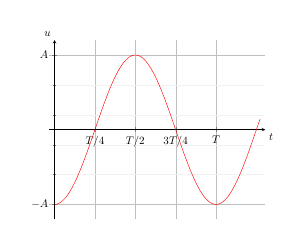
\begin{tikzpicture}[scale=0.4]
                \begin{axis}%
                    [grid=both,
                    minor tick num=4,
                    grid style={line width=.1pt, draw=gray!10},
                    major grid style={line width=.2pt,draw=gray!50},
                    axis lines=middle,
                    enlargelimits={abs=0.2},
                    xlabel={$t$},
                    ylabel={$u$},
                    xlabel style={below right},
                    ylabel style={above left},
                    xtick={pi/2,pi,3*pi/2, 2*pi},
                    xticklabels={$T/4$,$T/2$,$3T/4$,$T$},
                    ytick={-1,1},
                    yticklabels={$-A$,$A$}
                    ]
                    \addplot[domain=0:8,samples=100,smooth,red] {cos(deg(x+pi))};
                \end{axis}
            \end{tikzpicture}
        \end{column}

        \begin{column}{0.45\textwidth}
            \[\delta = \pi/2\]
            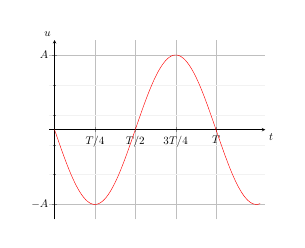
\begin{tikzpicture}[scale=0.4]
                \begin{axis}%
                    [grid=both,
                    minor tick num=4,
                    grid style={line width=.1pt, draw=gray!10},
                    major grid style={line width=.2pt,draw=gray!50},
                    axis lines=middle,
                    enlargelimits={abs=0.2},
                    xlabel={$t$},
                    ylabel={$u$},
                    xlabel style={below right},
                    ylabel style={above left},
                    xtick={pi/2,pi,3*pi/2, 2*pi},
                    xticklabels={$T/4$,$T/2$,$3T/4$,$T$},
                    ytick={-1,1},
                    yticklabels={$-A$,$A$}
                    ]
                    \addplot[domain=0:8,samples=100,smooth,red] {cos(deg(x+pi/2))};
                \end{axis}
            \end{tikzpicture}

            \[\delta = -\pi/2\]
            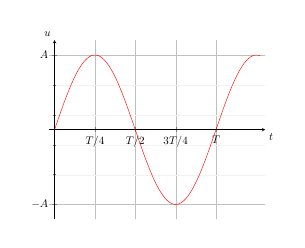
\begin{tikzpicture}[scale=0.4]
                \begin{axis}%
                    [grid=both,
                    minor tick num=4,
                    grid style={line width=.1pt, draw=gray!10},
                    major grid style={line width=.2pt,draw=gray!50},
                    axis lines=middle,
                    enlargelimits={abs=0.2},
                    xlabel={$t$},
                    ylabel={$u$},
                    xlabel style={below right},
                    ylabel style={above left},
                    xtick={pi/2,pi,3*pi/2, 2*pi},
                    xticklabels={$T/4$,$T/2$,$3T/4$,$T$},
                    ytick={-1,1},
                    yticklabels={$-A$,$A$}
                    ]
                    \addplot[domain=0:8,samples=100,smooth,red] {cos(deg(x-pi/2))};
                \end{axis}
            \end{tikzpicture}
        \end{column}
    \end{columns}
\end{frame}

\begin{frame}{Capítulo 15: Problema 1 modificado}
    \begin{minipage}{\textwidth}
        Um objeto que executa um movimento harmônico simples leva \SI{0.25}{s} para se deslocar de um ponto de
        velocidade nula para o ponto seguinte \textit{com velocidade nula}. A distância entre os pontos é \SI{36}{cm}. Calcule (a) o
        período, (b) a frequência e (c) a amplitude do movimento
    \end{minipage}
    \pause
    \begin{itemize}
    \color{blue}
        \item \(x=A\cos{\omega t} \implies v=-\omega A \sen{\omega t} \)
        \item \(v=0 \implies \omega t = 0 \text{ ou } \omega t = \pi \implies t = \pi /\omega\)
        \item \(T=2\pi / \omega \text{ e } \SI{0.25}{s} = \pi / \omega \implies T=2 \times \SI{0.25}{s} = \SI{0.50}{s}\)
        \item \(f=1/T \implies f=1/\SI{0.5}{s} = \SI{2}{s^{-1}} = \SI{2}{Hz}\)
        \item \(\omega t = 0 \text{ ou } \omega t = \pi \implies x_i=A \text{ e } x_f=A \implies \Delta x = 2A
            \implies 2A= \SI{36}{cm} \implies {A=\SI{18}{cm}}\)
    \end{itemize}
\end{frame}

\begin{frame}{Capítulo 15: mais problemas}
    \begin{itemize}
        \item Problemas 7, 8, 12 e 15
    \end{itemize}
\end{frame}

\begin{frame}{Pêndulo simples}
    \begin{columns}[T]
        \begin{column}{0.4\textwidth}
            \begin{tikzpicture}[scale=1/2,
                ground/.style={fill,pattern=north east lines,draw=none,minimum width=0.3,minimum height=0.6}
                ]
                \draw [ground] (0,0) rectangle (10,1);
                \draw [thick] (0,0) -- (10,0);
                \draw [dotted,thick] (5,0) -- (5,-8);
                \draw [thick] (5,0) -- ++(-60:8) node [midway, above right] {L} node [circle, fill=blue!10, draw=black] {m} coordinate (A);
                \draw [red,->] (A) ++(0,-0.5) -- ++(0,-1) node [below] {mg} ;
                \draw (5,-2) arc (270:300:2) node [midway, below] {$\theta$};
            \end{tikzpicture}
        \end{column}
        \begin{column}{0.45\textwidth}
            \begin{itemize}
                \item Temos que \(\tau = -Lmg \sen{\theta}\)
                \item \textit{Lembrando de Física I}, temos que
                    \[
                        I\alpha = \tau \implies I\frac{d^2 \theta}{dt^2} = -Lmg\sen{\theta}
                    \]
                \item Quando \(\theta \to 0\) temos \(\sen{\theta} \to \theta\) e assim
                    \[
                        \frac{d^2\theta}{dt^2} = - \frac{Lmg}{I}\theta
                    \]
                \item Ou seja
                    \begin{itemize}
                        \item para \(\theta\) grande não temos um MHS
                        \item para \(\theta\) pequeno temos um MHS
                    \end{itemize}
            \end{itemize}
        \end{column}

    \end{columns}
\end{frame}

\begin{frame}[c]{Pêndulo simples simplificado}
    Se pudermos considerar a massa do fio desprezível e a massa do corpo que oscila concentrada no centro de massa, temos que
    \(I=mL^2\) e assim temos a fórmula
    \[
        \omega = \sqrt{\frac{g}{L}}
    \]
\end{frame}

\begin{frame}{Exemplos}
    \begin{itemize}
        \item Problemas 33, 42 e 45
    \end{itemize}
\end{frame}

\begin{frame}{Problema 49}
    \begin{minipage}{\textwidth}
        O ângulo do pêndulo da figura abaixo é dado por
        \(\theta = \theta \cos{[(\SI{4.44}{rad/s})t+\phi]}\). Se, em \(t=0\), \(\theta=\SI{0.040}{rad}\)
        e \(d\theta/dt = \SI{-0.200}{rad/s}\), qual é (a) a constante de fase \(\phi\) e (b) qual é
        o ângulo máximo \(\theta_m\)?
    \end{minipage}
    \begin{center}
        \begin{tikzpicture}[scale=1/2,
            ground/.style={fill,pattern=north east lines,draw=none,minimum width=0.3,minimum height=0.6}
            ]
            \draw [ground] (0,0) rectangle (10,1);
            \draw [thick] (0,0) -- (10,0);
            \draw [dotted,thick] (5,0) -- (5,-8);
            \draw [thick] (5,0) -- ++(-60:8) node [midway, above right] {L} node [circle, fill=blue!10, draw=black] {m} coordinate (A);
            % \draw [red,->] (A) ++(0,-0.5) -- ++(0,-1) node [below] {mg} ;
            \draw (5,-2) arc (270:300:2) node [midway, below] {$\theta$};
        \end{tikzpicture}
    \end{center}
\end{frame}

\begin{frame}{Problema 82 modificado}
    \begin{minipage}{\textwidth}
        Um pêndulo simples, com \SI{20}{cm} de comprimento e \SI{5.0}{g} de massa, está suspenso
        em um carro de corrida que se move a uma velocidade constante de \SI{70}{m/s}, descrevendo
        uma circunferência com \SI{50}{m} de raio. Se o pêndulo sofre pequenas oscilações na direção
        radial em torno da posição de equilíbrio, qual é a frequência das oscilações?

        \vspace{2cm}
        Compare o valor obtido com o esperado caso o carro estivesse parado.
    \end{minipage}
\end{frame}

\begin{frame}{Atividade - Ondas sonoras}
    \begin{itemize}
        \item Vale 25\% da \(N_2\)
        \item Grupo de no máximo 2 alunos
        \item Faça uma pesquisa sobre Ondas Sonoras contendo:
            \begin{itemize}
                \item Relação entre velocidade do som e massa específica/elasticidade do meio de propagação
                \item Nível sonoro em decibéis
                \item O aparelho auditivo humano
            \end{itemize}
        \item Data de entrega 15/1
    \end{itemize}
\end{frame}

\begin{frame}{Movimento ondulatório}
    \begin{itemize}
        \item Uma \textbf{onda} surge quando um sistema é deslocado de sua \textit{posição}
            de equilíbrio e a \textbf{perturbação} se propaga de uma região para outra
            do sistema com \textbf{velocidade definida}
        \item Uma onda carrega energia mas, em geral, não carrega matéria
        \item Onda mecânica: precisa de um meio para se propagar
        \item Onda eletromagnética: não precisa de um meio para se propagar
    \end{itemize}
    \begin{center}
        \includegraphics[height=0.3\textwidth]{images/ondas_na_água.jpg}
    \end{center}
\end{frame}

\begin{frame}
    \begin{itemize}
        \item Onda \textbf{longitudinal}: a perturbação ocorre \textbf{paralela} à direção
            de propagação

        \item Onda \textbf{transversal}: a perturbação ocorre \textbf{perpendicular} à direção
            de propagação
    \end{itemize}

    \vspace{1cm}
    \centering
    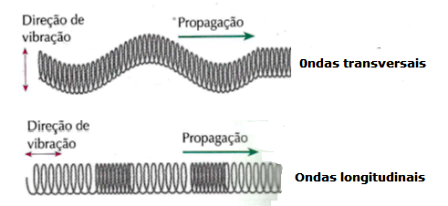
\includegraphics[height=0.6\textheight]{images/onda_lon_tra.png}
\end{frame}

\begin{frame}{Função de onda}
    \begin{itemize}
        \item Chamamos de \textbf{função de onda} a representação matemática de uma onda
        \item Todas as funções de onda são soluções da equação diferencial
            \[
                \frac{\partial^2 y}{\partial x^2} = 
                \frac{1}{v^2} \frac{\partial^2 y}{\partial t^2}
            \]
            onde \(v\) é a velocidade de propagação da onda
        \item Com um pouco de imaginação, podemos ver que qualquer função
            \(y=f(x \pm vt)\) é uma função de onda, onde:
            \begin{align*}
                y&=f(x-vt) \implies \text{onda se movendo no sentido } +x \\
                y&=f(x+vt) \implies \text{onda se movendo no sentido } -x 
            \end{align*}
    \end{itemize}
\end{frame}

\begin{frame}{Ondas harmônicas}
    \begin{itemize}
        \item Uma onda é harmônica se tem a forma
            \[
                y=A \cos{(kx \pm \omega t+ \delta)}
            \]
            onde
            \begin{itemize}
                \item \(A\) é a amplitude
                \item \(k\) é o número de onda, que se relaciona ao comprimento de onda 
                    \(\lambda\) pela fórmula
                    \[
                        \lambda = \frac{2\pi}{k}
                    \]
                \item \(\omega\) é a frequência angular que se relaciona ao período \(T\)
                    e a frequência \(f\) pelas fórmulas
                    \[
                        T=\frac{2\pi}{\omega} \qquad f=\frac{\omega}{2\pi}
                    \]
                \item \(\delta\) é a constante de fase
            \end{itemize}
        \item Pode-se verificar que
            \[
                {\color{blue} v=\frac{\omega}{k}} \text{ ou } {\color{red} v=\lambda f}
            \]
    \end{itemize}

\end{frame}

\begin{frame}{Atividade}
    Exercícios do capítulo 16: 9, 10, 13, 29, 30, 66, 70 e 73
\end{frame}
